\documentclass[paper=a4, fontsize=11pt]{scrartcl}
\usepackage[T1]{fontenc}
\usepackage{fourier}

\usepackage[english]{babel}															% English language/hyphenation
\usepackage[protrusion=true,expansion=true]{microtype}	
\usepackage{amsmath,amsfonts,amsthm} % Math packages
\usepackage[pdftex]{graphicx}	
\usepackage{url}
\usepackage{hyperref}


%%% Custom sectioning
\usepackage{sectsty}
\allsectionsfont{\centering \normalfont\scshape}
\usepackage{subfigure}

\usepackage{comment}


%%% Custom headers/footers (fancyhdr package)
\usepackage{fancyhdr}
\pagestyle{fancyplain}
\fancyhead{}											% No page header
\fancyfoot[L]{}											% Empty 
\fancyfoot[C]{}											% Empty
\fancyfoot[R]{\thepage}									% Pagenumbering
\renewcommand{\headrulewidth}{0pt}			% Remove header underlines
\renewcommand{\footrulewidth}{0pt}				% Remove footer underlines
\setlength{\headheight}{13.6pt}


%%% Equation and float numbering
%\numberwithin{equation}{section}		% Equationnumbering: section.eq#
%\numberwithin{figure}{section}			% Figurenumbering: section.fig#
%\numberwithin{table}{section}				% Tablenumbering: section.tab#


%%% Maketitle metadata
\newcommand{\horrule}[1]{\rule{\linewidth}{#1}} 	% Horizontal rule

\title{
		%\vspace{-1in} 	
		\usefont{OT1}{bch}{b}{n}
		\normalfont \normalsize \textsc{CS650 - Computer Vision} \\ [25pt]
		\horrule{0.5pt} \\[0.4cm]
		\huge Programming Lab 2 \\ Edge Detection / Hough Transform \\
		\horrule{2pt} \\[0.5cm]
}
\author{
		\normalfont 								\normalsize
        Daqing Yi\\[-3pt]		\normalsize
        \today
}
\date{}


%%% Begin document
\begin{document}
\maketitle

\begin{comment}
Prepare a brief writeup that includes each part and submit it as a PDF through Canvas.
Your writeup should document your findings for Part 1 but otherwise focus on your methods and results for Part 2.

Note: many of the images for Part 1 will contain negative numbers or numbers larger than 255.
Make sure you appropriately scale the output images to display all of the information.
(Hint: if there are negative values, try mapping 0 to 128 with positive values mapped to the range (128,255] and negative values to the range [0,128).]
\end{comment}

This lab consists of two parts, edge detection and hough transform.
The implementations are written in Python.
PIL is used for reading image files into data arrays.
Numpy is used for array operations.
Matplotlib and imshow (from openCV) is used for visualizing data.

\section{Edge detection}

Edge detection aims at finding the edges inside the images by the clues.
The representation is usually a set of points.
The implementation is in \emph{EdgeDetection.py}.

\subsection{First and Second Order Derivatives of an Image}

\begin{figure}[h]
\centering
\subfigure[Origin]{
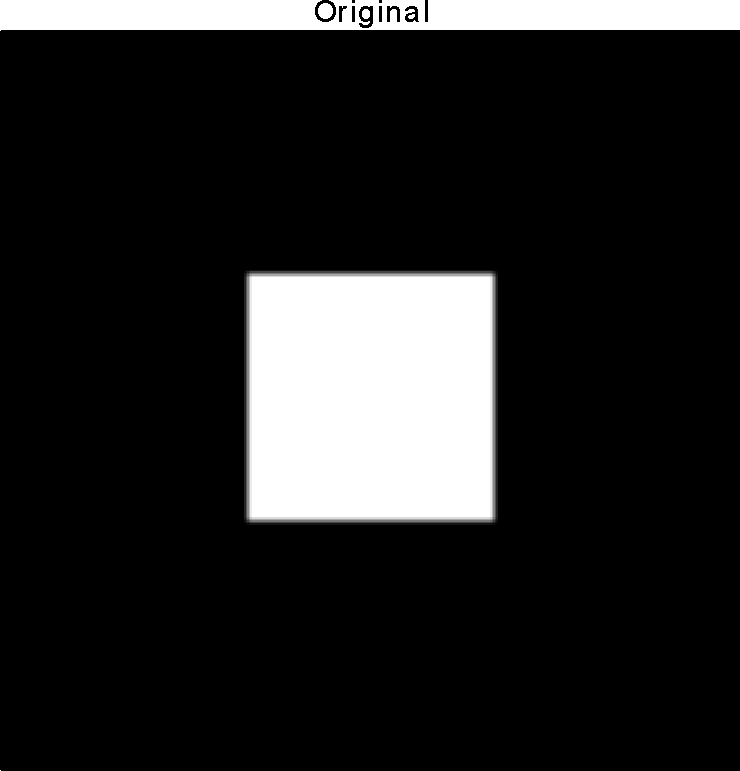
\includegraphics[width=.23\textwidth]{./figure/2D_White_Box_origin}
\label{fig:edge:01:origin} }
\subfigure[Gradient Magnitude]{
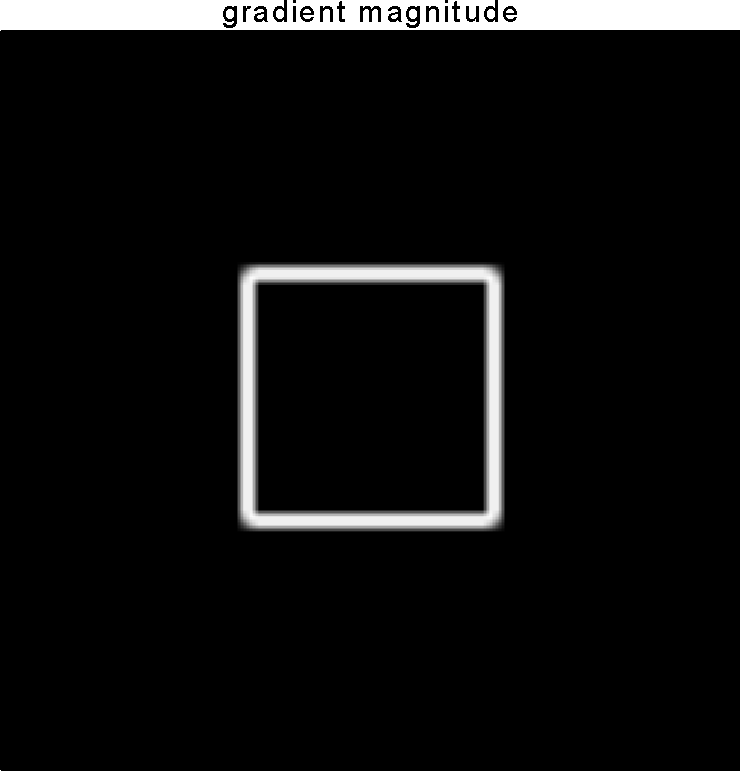
\includegraphics[width=.23\textwidth]{./figure/2D_White_Box_gradient_magnitude} 
\label{fig:edge:01:gradient_magnitude} }
\subfigure[Gradient Orientation]{
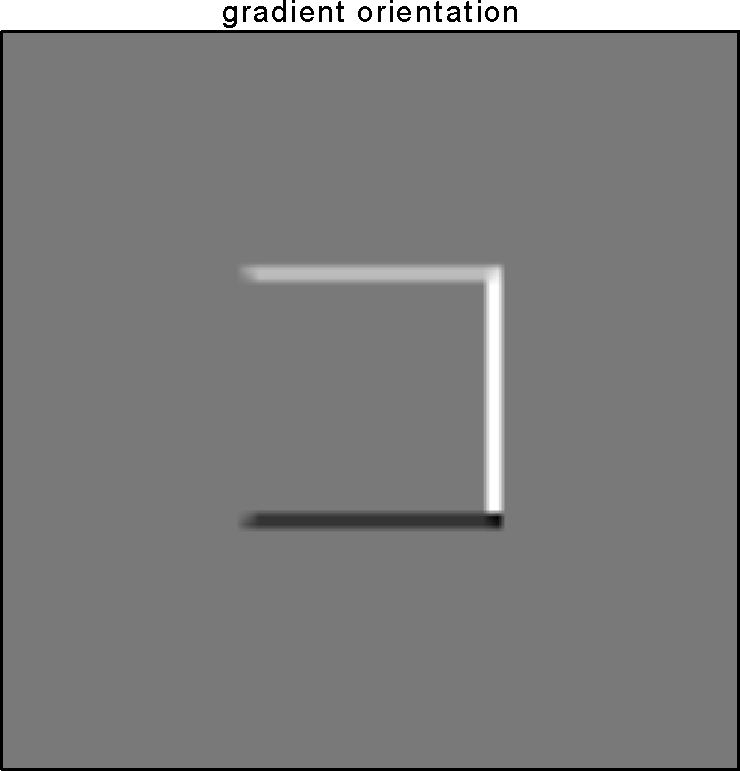
\includegraphics[width=.23\textwidth]{./figure/2D_White_Box_gradient_orientation}
\label{fig:edge:01:gradient_orientation} }
\subfigure[Laplacian]{
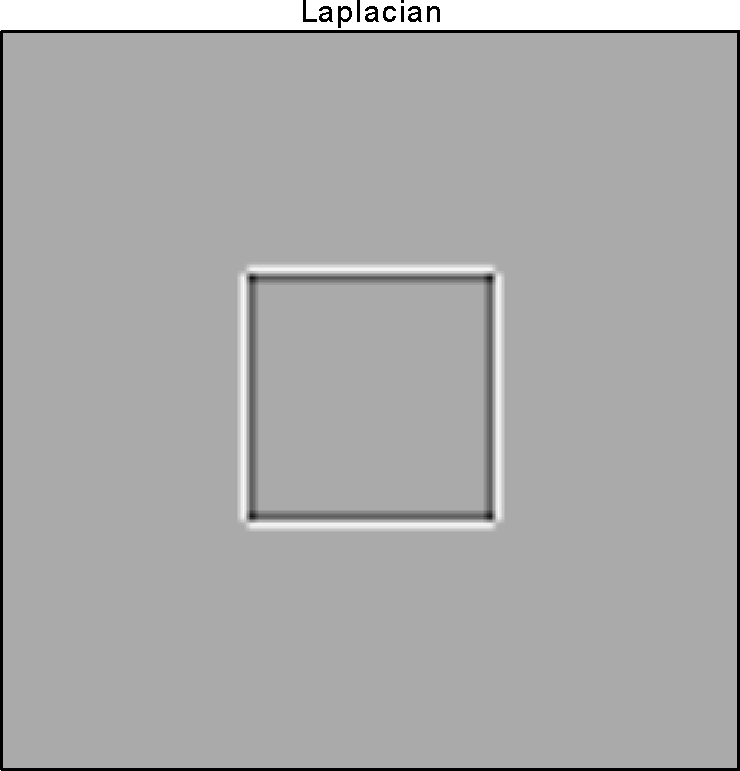
\includegraphics[width=.23\textwidth]{./figure/2D_White_Box_laplacian} 
\label{fig:edge:01:laplacian} }
\caption{Derivatives of \emph{2D\_White\_Box.pgm} by 1st order and 2nd order.}
\label{fig:edge:01}
\end{figure}

The clues for finding the edges are obtained from differential geometry.
Figure \ref{fig:edge:01} and Figure \ref{fig:edge:02} give the examples on 1st order and 2nd order derivatives.
Figure \ref{fig:edge:01:gradient_magnitude} and Figure \ref{fig:edge:02:gradient_magnitude} illustrate the gradient magnitude, which shows the strength of intensity variation of each pixel.
Figure \ref{fig:edge:01:gradient_orientation} and Figure \ref{fig:edge:02:gradient_orientation} provide the gradient orientation, which provides the direction of intensity variation of each pixel.
Figure \ref{fig:edge:01:laplacian} and Figure \ref{fig:edge:02:laplacian} offer the 2nd derivatives, which can be used to identify the local maximum or minimum.

\begin{figure}[h]
\centering
\subfigure[Origin]{
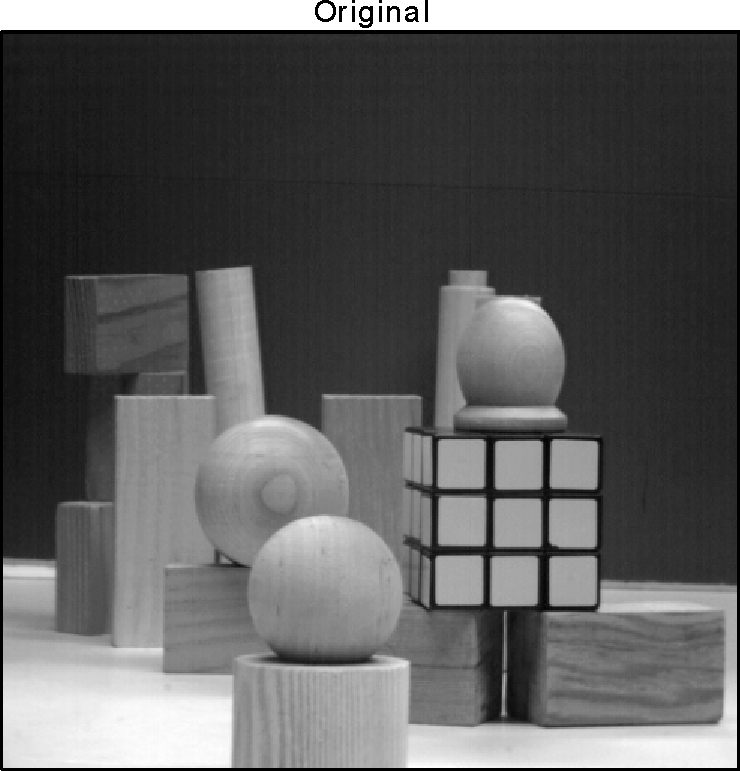
\includegraphics[width=.23\textwidth]{./figure/blocks_origin}
\label{fig:edge:02:origin} }
\subfigure[Gradient Magnitude]{
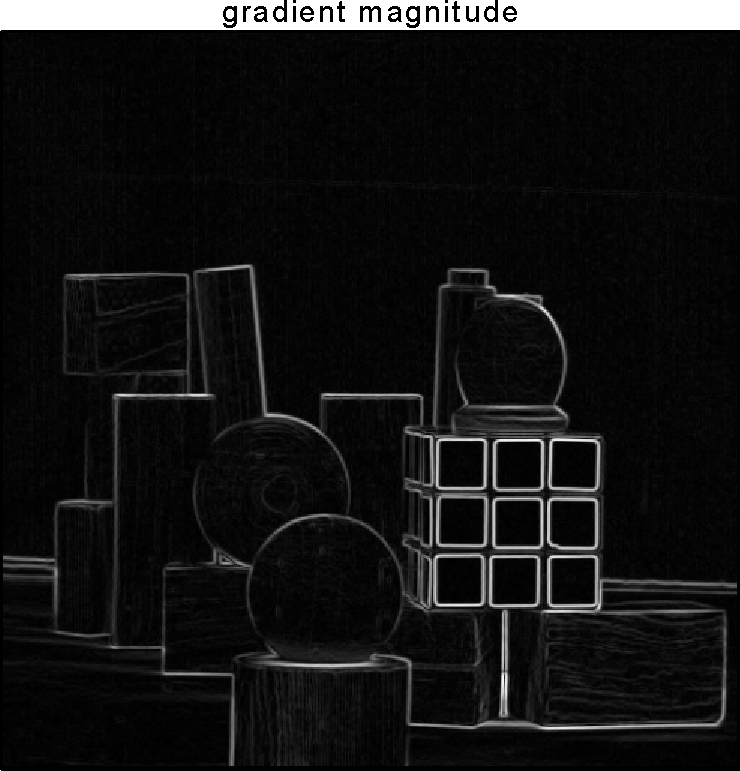
\includegraphics[width=.23\textwidth]{./figure/blocks_gradient_magnitude} 
\label{fig:edge:02:gradient_magnitude} } 
\subfigure[Gradient Orientation]{
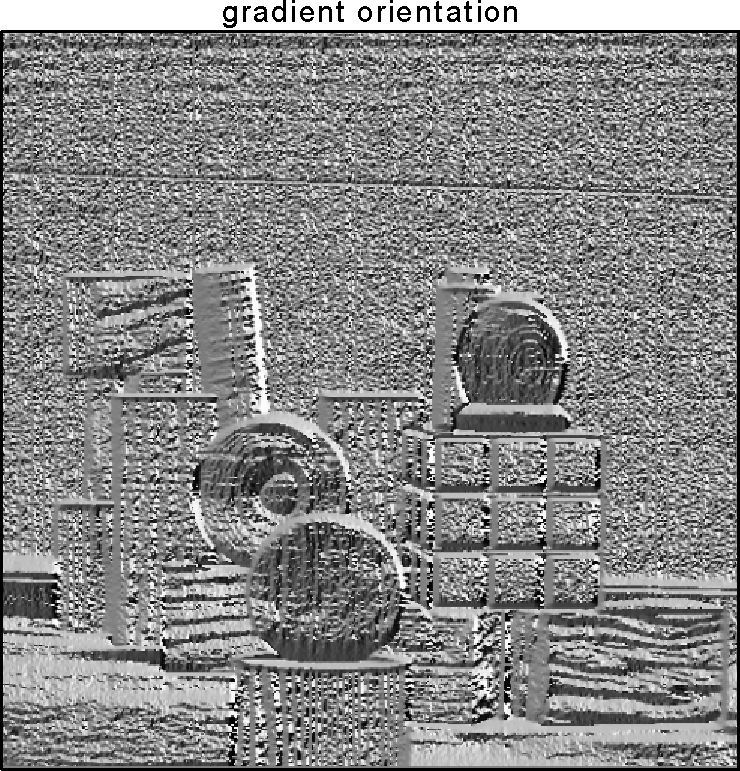
\includegraphics[width=.23\textwidth]{./figure/blocks_gradient_orientation}
\label{fig:edge:02:gradient_orientation} }
\subfigure[Laplacian]{
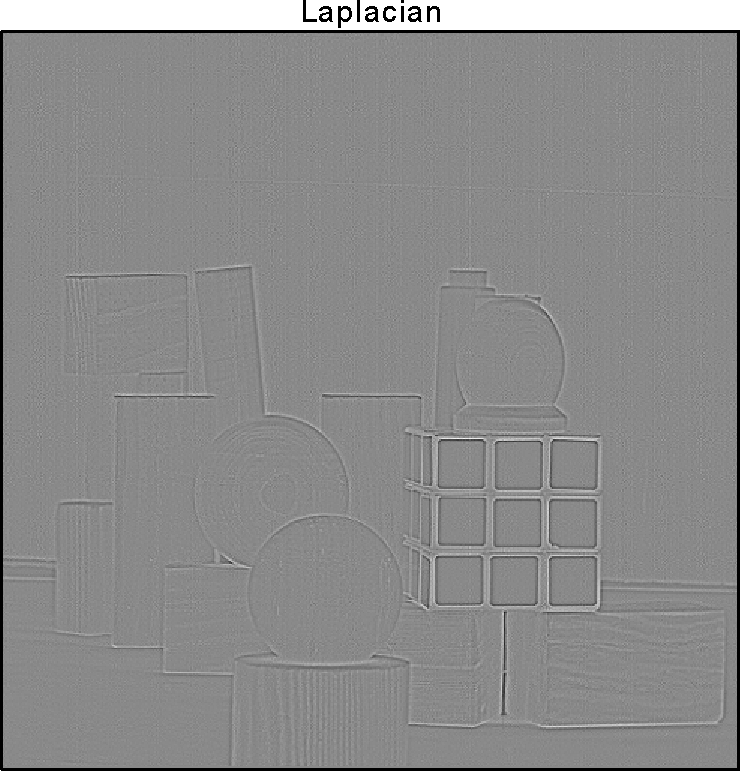
\includegraphics[width=.23\textwidth]{./figure/blocks_laplacian} 
\label{fig:edge:02:laplacian} }
\caption{Derivatives of \emph{blocks.pgm} by 1st order and 2nd order.}
\label{fig:edge:02}
\end{figure}

\subsection{edge detection}

With the clues given, edge detection methods can be applied.
Two types of methods are implemented in \emph{EdegDetection.py}, which are \textbf{canny edge detector} and \textbf{zero-crossing edge detector}.

\subsubsection{Canny edge detector}

Canny edge detector is implemented in \emph{canny} in \emph{EdegDetection.py}.
Methods \emph{nonmaximalSuppresion()} and \emph{gaussianFilter()} are used to preprocess before applying the threshold binarization.
\emph{gaussianFilter()} can smooth the distribution.
\emph{nonmaximalSuppresion()} can thinner the cluster of the points by comparing the neighborhood.
It relies on the gradient orientation.
A \emph{hysteresisThreshold()} is applied for binarization based on the gradient magnitude.
A pixel above the low threshold but below the high threshold needs checking its connected pixels in determining whether it is an edge point.


\begin{figure}[h]
\centering
\subfigure[hi\_threshod=40, lo\_threshod=20]{
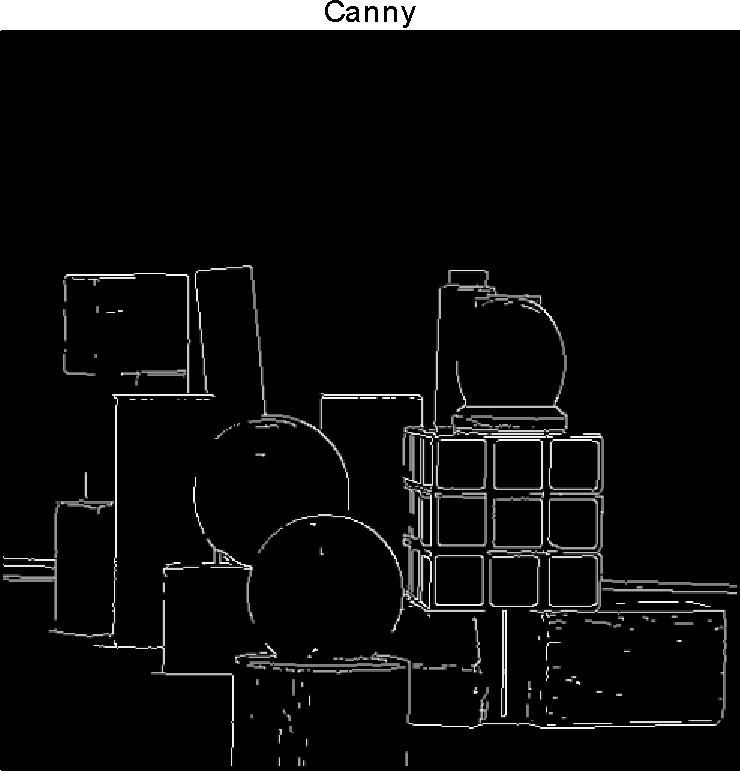
\includegraphics[width=.235\textwidth]{./figure/blocks_canny_20_40}
\label{fig:edge:02:canny:1} }
\subfigure[hi\_threshod=60, lo\_threshod=30]{
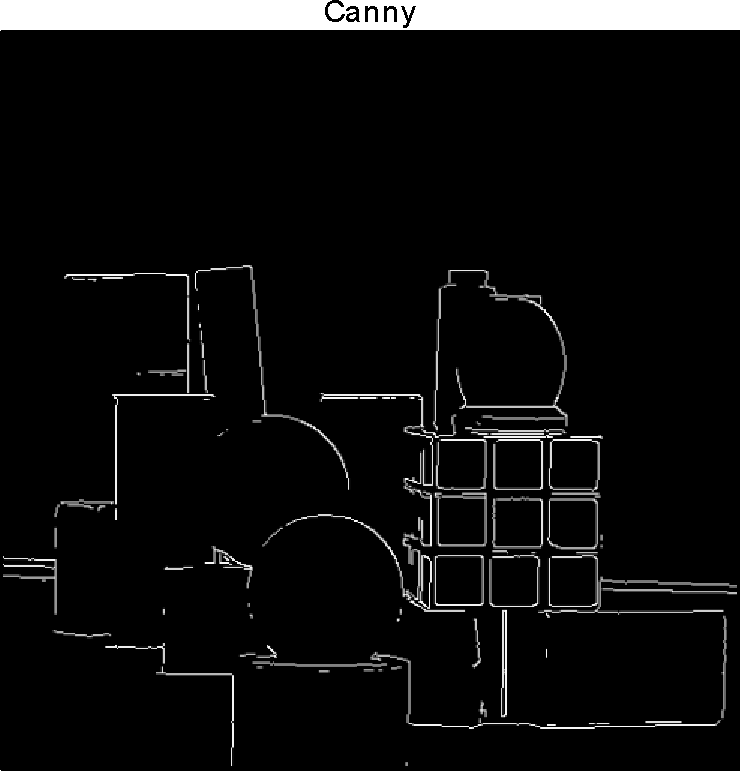
\includegraphics[width=.235\textwidth]{./figure/blocks_canny_30_60} 
\label{fig:edge:02:canny:2} } 
\subfigure[hi\_threshod=80, lo\_threshod=40]{
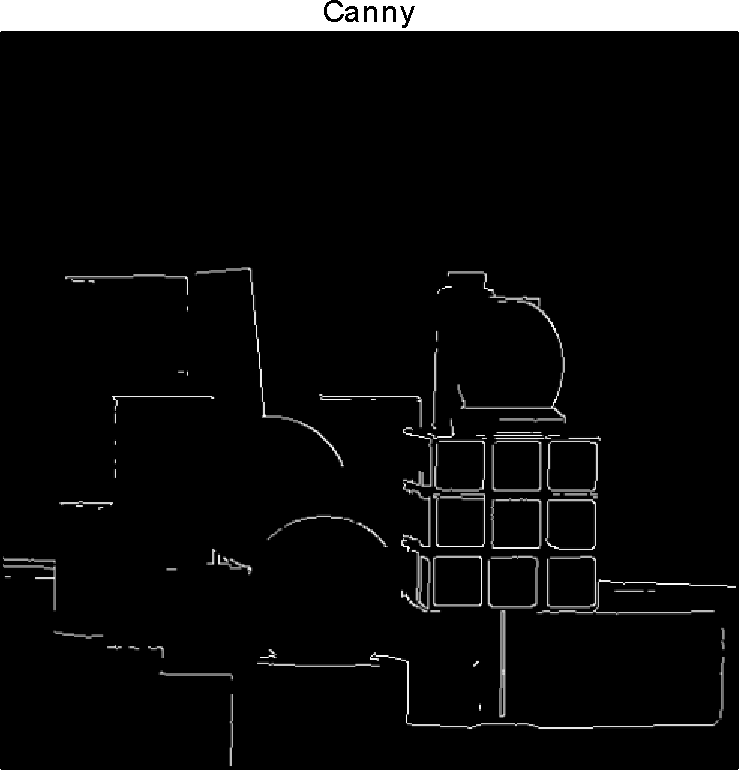
\includegraphics[width=.235\textwidth]{./figure/blocks_canny_40_80}
\label{fig:edge:02:canny:3} }
\subfigure[hi\_threshod=60, lo\_threshod=30, with Gaussian filter]{
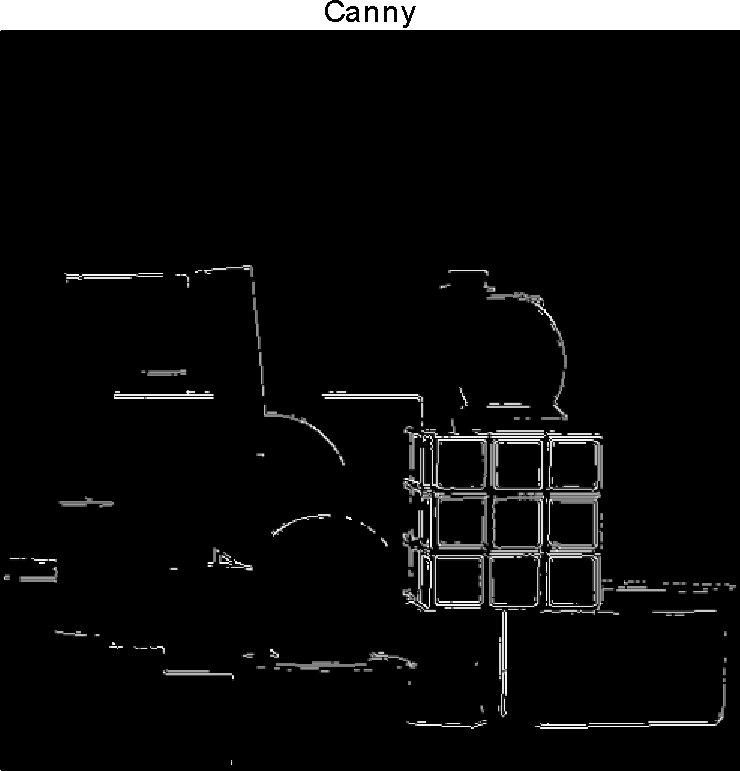
\includegraphics[width=.235\textwidth]{./figure/blocks_canny_gauss_30_60} 
\label{fig:edge:02:canny:gauss} }
\caption{Canny edge detector on \emph{blocks.pgm} using different parameters.}
\label{fig:edge:02:canny}
\end{figure}

Different parameters are tried. 
The difference on the edges found are illustrated in Figure \ref{fig:edge:02:canny}.
Lowering the low threshold tends to connect the disconnected edges.
Increasing the high threshold decreases the edge details that can be found.

\subsection{Laplacian zero-crossing edge detector}

A variant of canny edge detector uses the zero-crossing of the 2nd derivatives.
Because it is linked to Marr$-$Hildreth (zero crossing of the Laplacian) edge detector \footnote{\url{http://en.wikipedia.org/wiki/Canny_edge_detector}}, the function name is chosen as \emph{mh()} in \emph{EdgeDetection.py}.

\begin{figure}[h]
\centering
\subfigure[Threshold=40]{
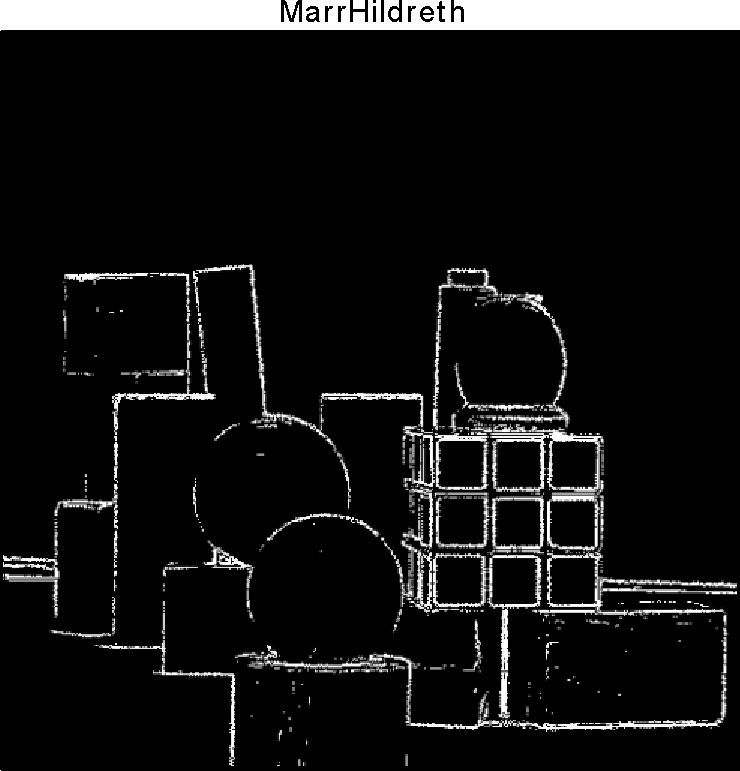
\includegraphics[width=.235\textwidth]{./figure/blocks_mh_40}
\label{fig:edge:02:mh:1} }
\subfigure[Threshold=60]{
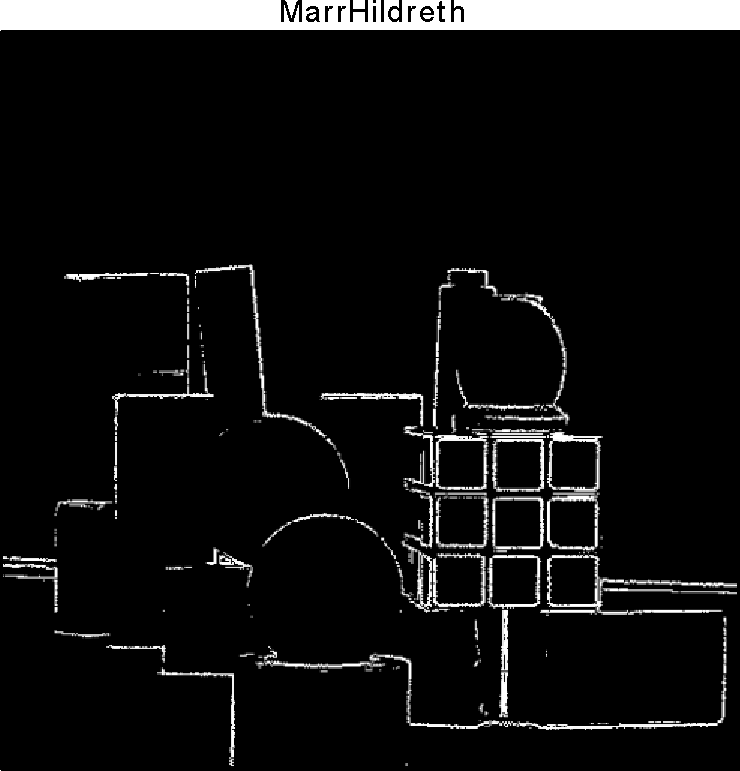
\includegraphics[width=.235\textwidth]{./figure/blocks_mh_60} 
\label{fig:edge:02:mh:2} } 
\subfigure[Threshold=80]{
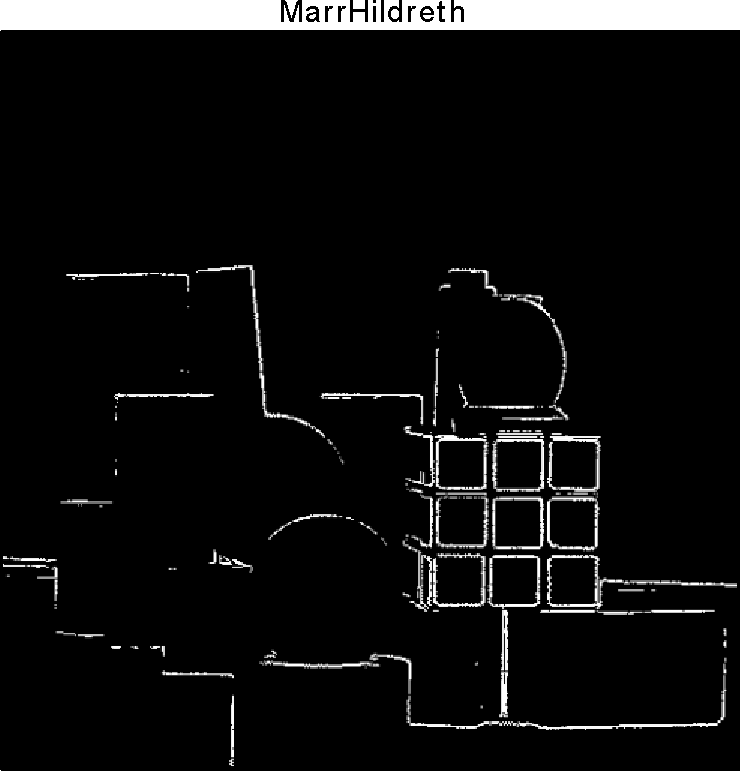
\includegraphics[width=.235\textwidth]{./figure/blocks_mh_80}
\label{fig:edge:02:mh:3} }
\subfigure[Threshold=40, with Gaussian filter]{
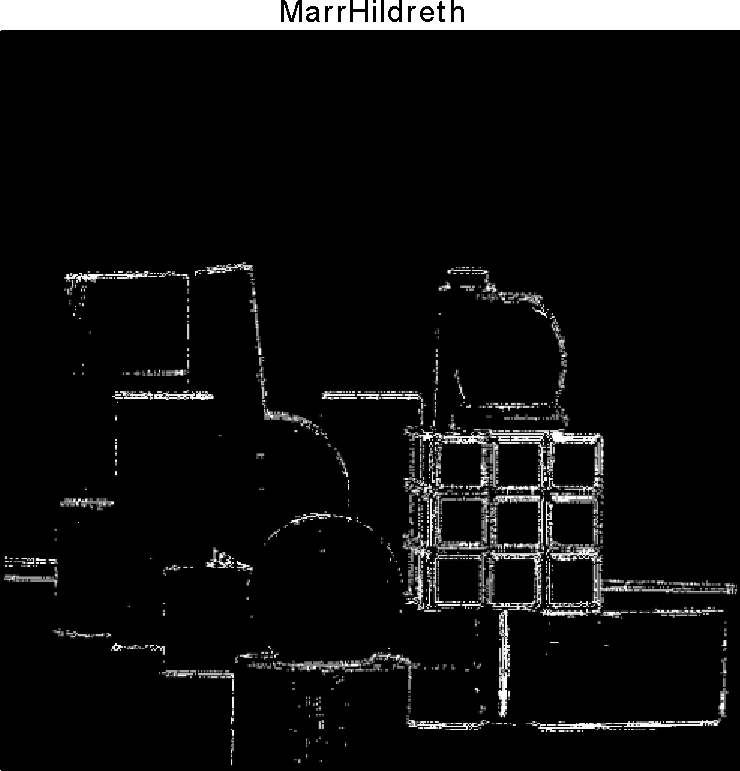
\includegraphics[width=.235\textwidth]{./figure/blocks_mh_gauss_40} 
\label{fig:edge:02:mh:gauss} }
\caption{Laplacian zero-crossing edge detector on \emph{blocks.pgm} using different parameters.}
\label{fig:edge:02:mh}
\end{figure}

This method checks whether there exists a zero crossing in a pixel along the direction of the gradient orientation.
If the pixel is a zero-crossing point, it means that it is likely to be a local maximum or minimum. 
A threshold is also applied here to filter some levels of noise.
Increasing the threshold removes the noise and small details, which is illustrated in Figure \ref{fig:edge:02:mh}.

\subsection{Discussion}

\begin{itemize}
\item \emph{Threshold determines the levels of details.} \\
Sliding the threshold can help finding the edge details needed in different applications.
The difference is illustrated in Figure \ref{fig:edge:02:canny} and Figure \ref{fig:edge:02:mh}.
\item \emph{Apply smooth filter only when necessary. } \\
Figure \ref{fig:edge:02:mh:gauss} gives an example.
When the picture has not a lot of noise, applying inappropriate smooth filter only bring side effects to edge detection.
\end{itemize}

\section{Hough transformation}

Hough transform is used for finding the features from detected edges.
It tries to find the points in the parameter space that maximize the likelihood of the distribution of the edge points.
From an edge point, all possible solutions in the parameter space could be found.
By accumulating all the possible parameters, we can have a parameter that connects to more edge points with a relatively higher value.
The local maximum then are chosen as the features found in the hough space.

\subsection{Hough circle transformation}

This lab aims at finding the circles in the pictures. 
Only three radii are tried, which are $ 16 $, $ 32 $ and $ 48 $ respectively.
Thus only two parameters, which are the x-coordinate and the y-coordinate of the centers of the circles, are left to explore.
The implementation is in \emph{HoughTransform.py}.
\emph{houghCircle()} provides a 2-D array for the accumulations of two parameters, which can be visualized into a 2-D image for the hough space.

\emph{simple\_circle.pgm} provides a simple case to verify the correctness of the function. 
Figure \ref{fig:hough:simple_circle} gives the process of finding the simple circle using a radius of 32.
The center found by running the code is $ (124, 127) $.

\begin{figure}[h]
\centering
\subfigure[Edges]{
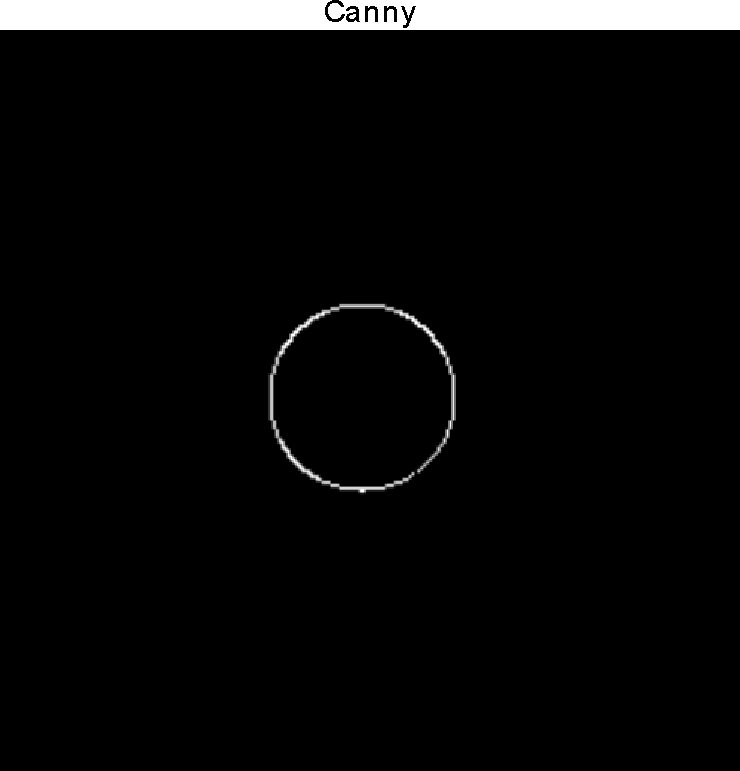
\includegraphics[width=.31\textwidth]{./figure/simplecircles_ppm_canny}
\label{fig:hough:simple_circle:edge} }
\subfigure[Hough space]{
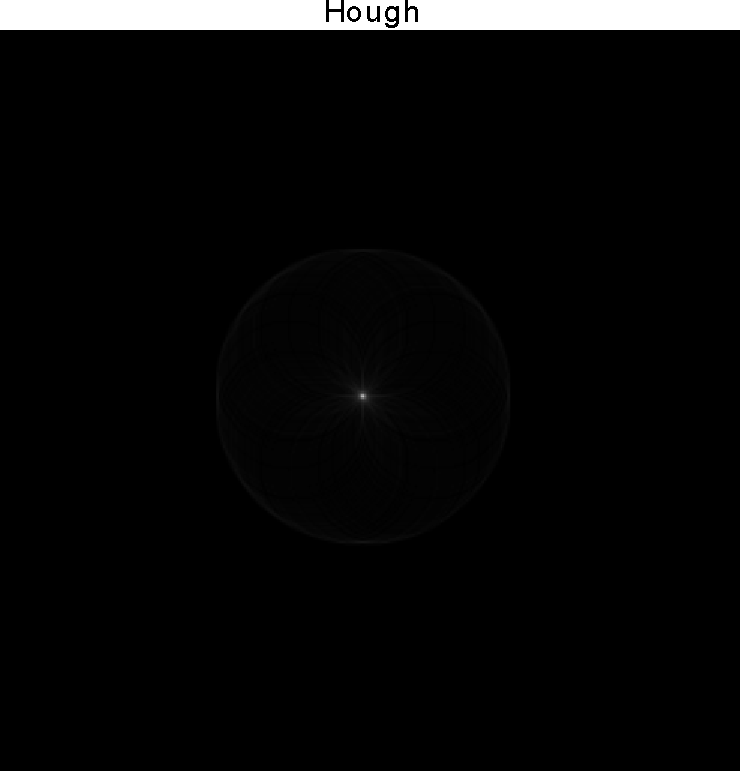
\includegraphics[width=.31\textwidth]{./figure/simplecircles_ppm_hough} 
\label{fig:hough:simple_circle:hough} } 
\subfigure[Circles found]{
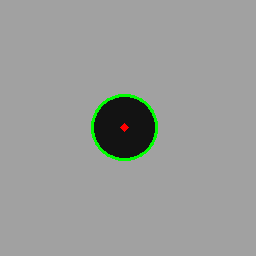
\includegraphics[width=.31\textwidth]{./figure/simplecircles_ppm_circles}
\label{fig:hough:simple_circle:circles} }
\caption{Detecting circles (radius=32) on \emph{circles.ppm}.}
\label{fig:hough:simple_circle}
\end{figure}

\subsection{Finding different circle features}

\emph{circles.ppm} is used to test the features finding capability in an image mixed with a lot of different features and additive noise.
Because the centers of some circles might locate outside of the image.
If the image size is (img\_width, img\_height), a range of [-radius, img\_width + radius] will be scanned for the x coordinate and a range of [-radius, img\_height + radius ] will be scanned for the y coordinate.
The test results are as following.
\begin{itemize}
\item radius = 16 : The centers of the circles found are (89, 115), (-7, 122), (28, 144), (28, 149), (25, 150), (90, 196), (52, 197) .
They are shown in Figure \ref{fig:hough:circle:16:circles}.
\item radius = 32 : The centers of the circles found are (46, 32), (57, 34), (150, 34), (220, 37), (158, 67), (79, 102), (89, 115), (173, 189), (186, 208) .
They are shown in Figure \ref{fig:hough:circle:32:circles}.
\item radius = 48 : The centers of the circles found are  (0, 103), (0, 108), (89, 115), (71, 206) .
They are shown in Figure \ref{fig:hough:circle:48:circles}.
\end{itemize}

\begin{figure}[h]
\centering
\subfigure[Edges]{
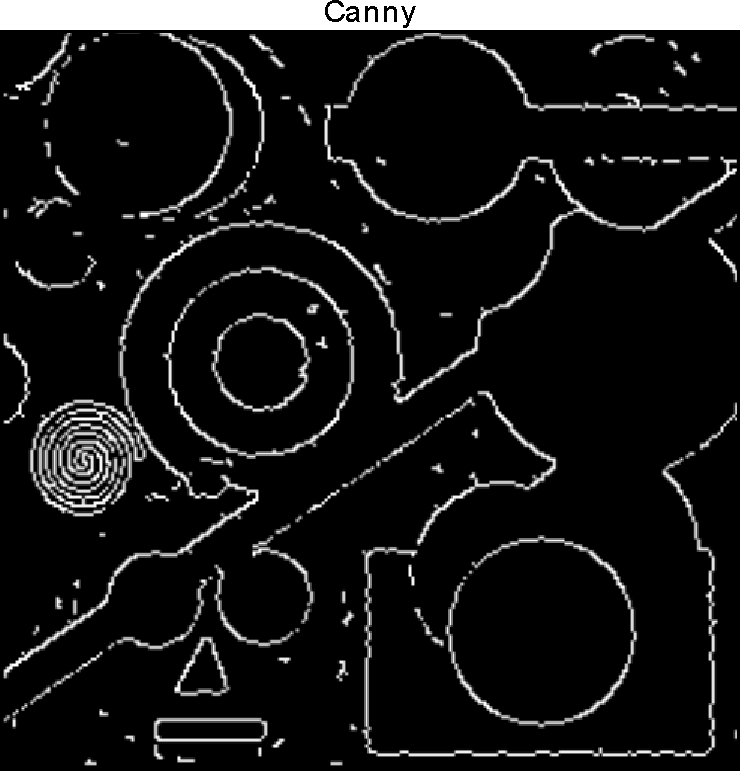
\includegraphics[width=.31\textwidth]{./figure/circles_ppm_canny_16}
\label{fig:hough:circle:16:edge} }
\subfigure[Hough space]{
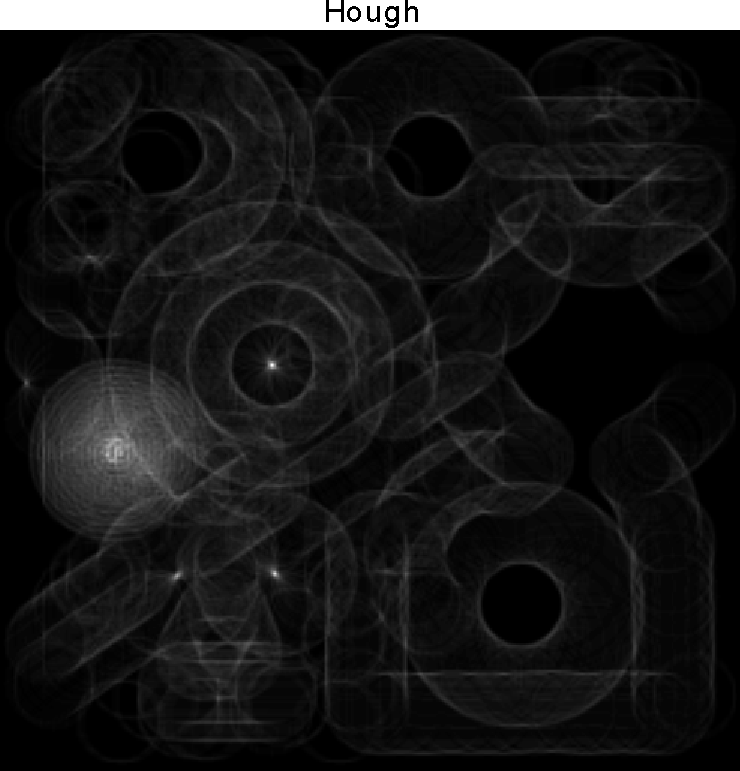
\includegraphics[width=.31\textwidth]{./figure/circles_ppm_hough_16} 
\label{fig:hough:circle:16:hough} } 
\subfigure[Circles found]{
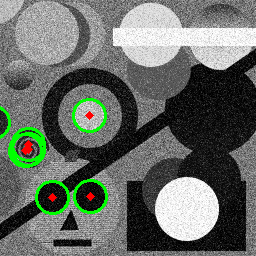
\includegraphics[width=.31\textwidth]{./figure/circles_ppm_circles_16}
\label{fig:hough:circle:16:circles} }
\caption{Detecting circles (radius=16) on \emph{circles.ppm}.}
\label{fig:hough:circle:16}
\end{figure}


\begin{figure}[h]
\centering
\subfigure[Edges]{
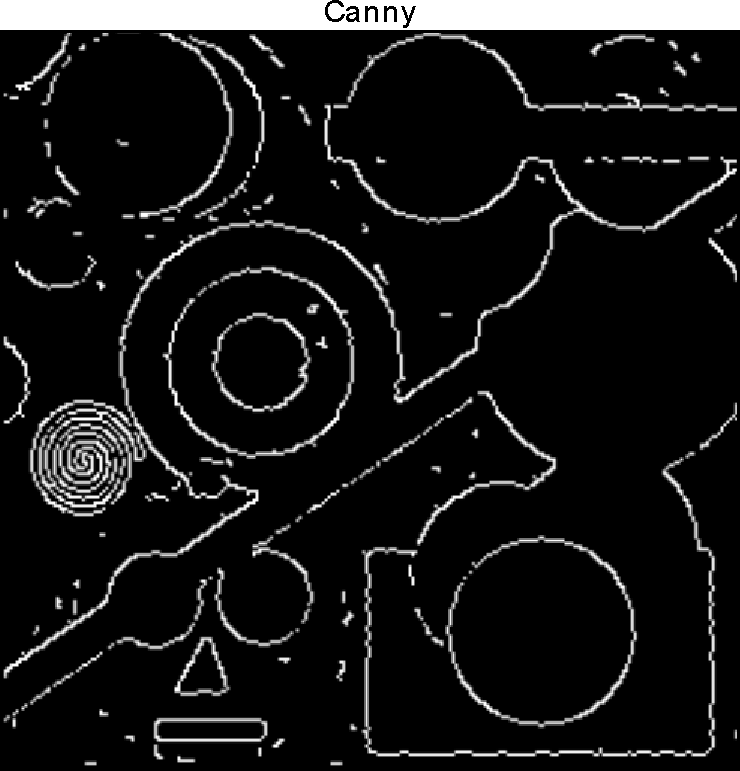
\includegraphics[width=.31\textwidth]{./figure/circles_ppm_canny_32}
\label{fig:hough:circle:32:edge} }
\subfigure[Hough space]{
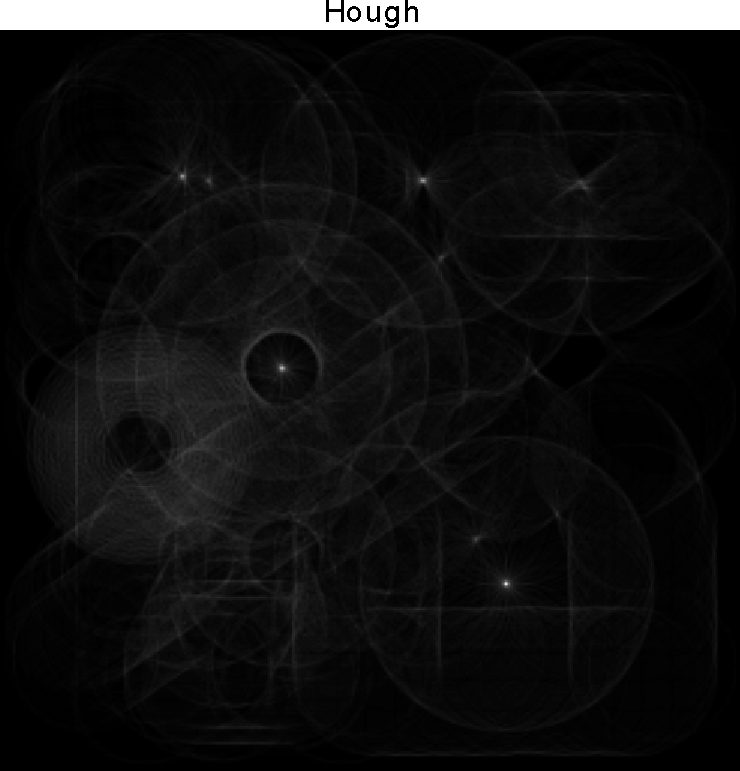
\includegraphics[width=.31\textwidth]{./figure/circles_ppm_hough_32} 
\label{fig:hough:circle:32:hough} } 
\subfigure[Circles found]{
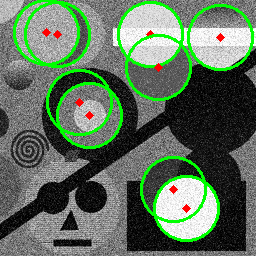
\includegraphics[width=.31\textwidth]{./figure/circles_ppm_circles_32}
\label{fig:hough:circle:32:circles} }
\caption{Detecting circles (radius=32) on \emph{circles.ppm}.}
\label{fig:hough:circle:32}
\end{figure}

\begin{figure}[h]
\centering
\subfigure[Edges]{
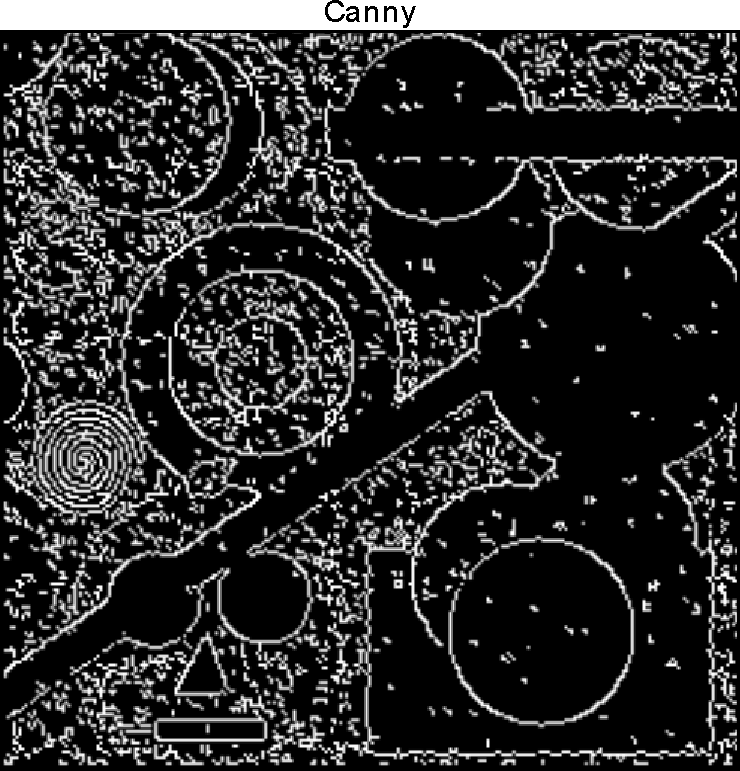
\includegraphics[width=.31\textwidth]{./figure/circles_ppm_canny_48}
\label{fig:hough:circle:48:edge} }
\subfigure[Hough space]{
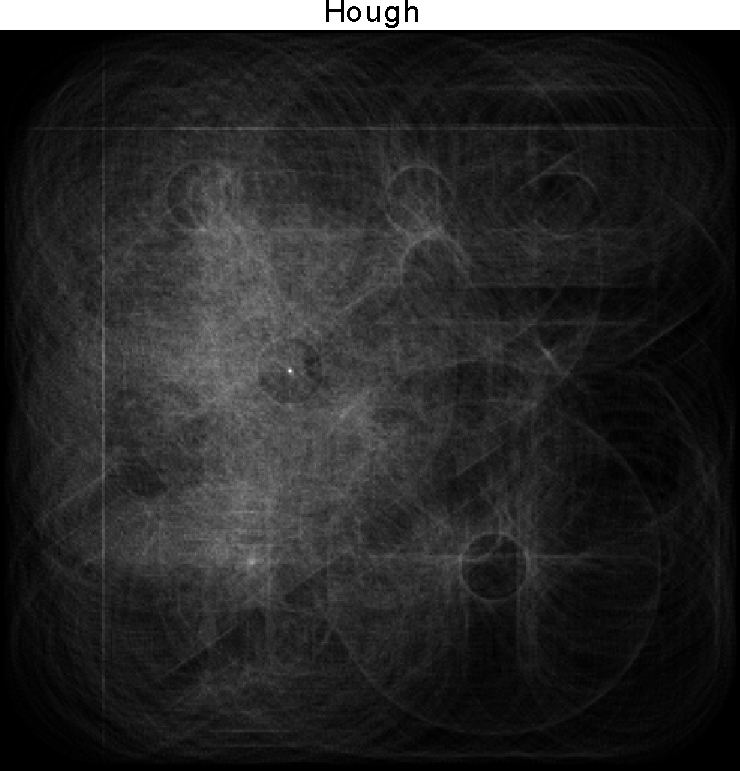
\includegraphics[width=.31\textwidth]{./figure/circles_ppm_hough_48} 
\label{fig:hough:circle:48:hough} } 
\subfigure[Circles found]{
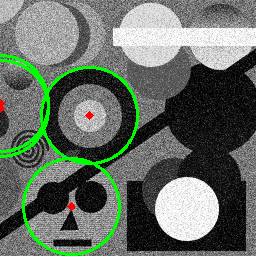
\includegraphics[width=.31\textwidth]{./figure/circles_ppm_circles_48}
\label{fig:hough:circle:48:circles} }
\caption{Detecting circles (radius=48) on \emph{circles.ppm}.}
\label{fig:hough:circle:48}
\end{figure}

Figure \ref{fig:hough:circle:16}, Figure \ref{fig:hough:circle:32} and Figure \ref{fig:hough:circle:48} provide the visualized processes and results of finding circles with different radii.
By human's visual experience, it is obvious that whether the circles are easy to tell depends on the edges detected.
In order to enhance the performance of edge detection, different parameters are applied to edge detection so that different patterns of edges could be detected.

\subsection{Apply different threshold for the centers outside of the image}

Because the center outside the image tends to make less edge points in the image, applying same threshold to these regions might miss some circles. 
Thus I tried to apply a different threshold in finding the local maximum in the region outside of the image.
The result on radius = 32 is tested and given.
The centers of the circles found are (-7, -8), (200, -4), (150, 34), (220, 37), (158, 67), (199, 116), (208, 178), (173, 189), (186, 208) .
As it is shown in Figure \ref{fig:hough:circle:32:cv:circles}, some circles that have the center outside of the image can also be found.

\begin{figure}[h]
\centering
\subfigure[Edges]{
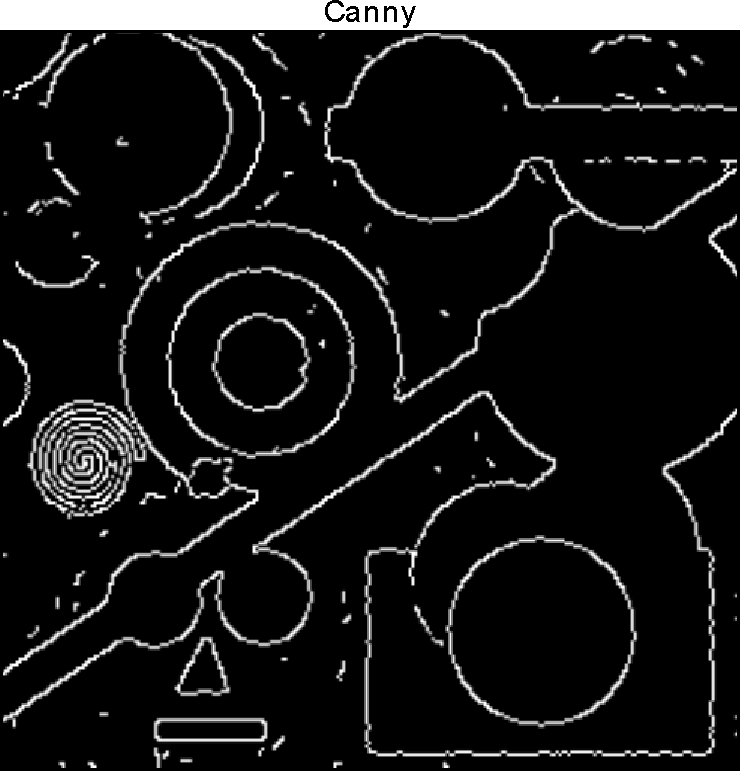
\includegraphics[width=.31\textwidth]{./figure/circles_ppm_canny_32_cv}
\label{fig:hough:circle:32:cv:edge} }
\subfigure[Hough space]{
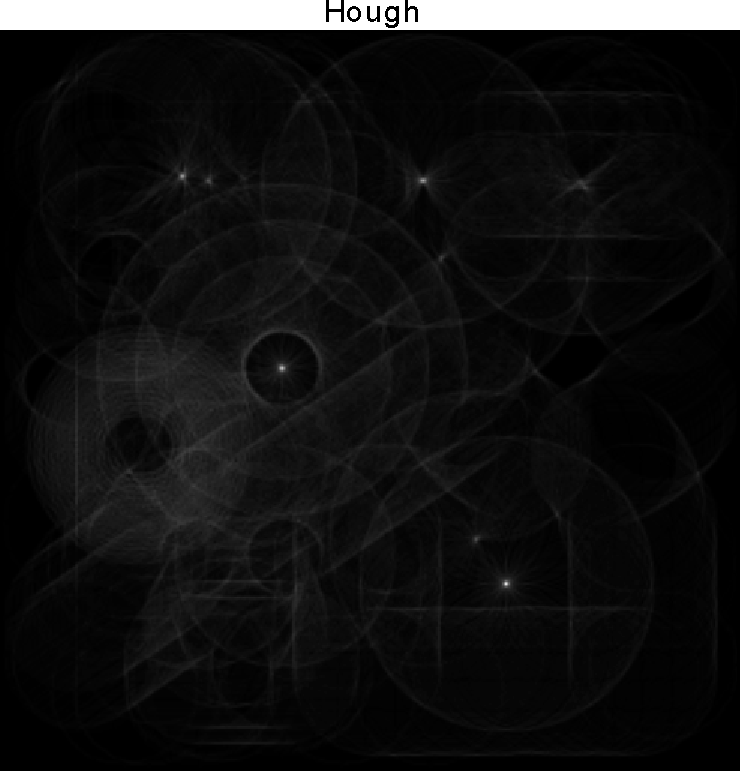
\includegraphics[width=.31\textwidth]{./figure/circles_ppm_hough_32_cv} 
\label{fig:hough:circle:32:cv:hough} } 
\subfigure[Circles found]{
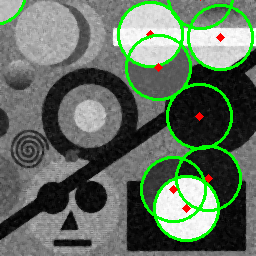
\includegraphics[width=.31\textwidth]{./figure/circles_ppm_circles_32_cv}
\label{fig:hough:circle:32:cv:circles} }
\caption{Detecting circles (radius=32) on \emph{circles.ppm} using different threshold for accumulators locating outside the image.}
\label{fig:hough:circle:32:cv}
\end{figure}

\subsection{Apply weighted revote}

The local maximum finding is not easy to support multiple radii (when a set of radii is given).
Weighted revoting described in the slides is tried as well.
Because the weights usually converge quickly.
Instead of checking weight convergence, I only run a fixed number of iterations in the revote process for simplicity.

\begin{figure}[h]
\centering
\subfigure[Hough space]{
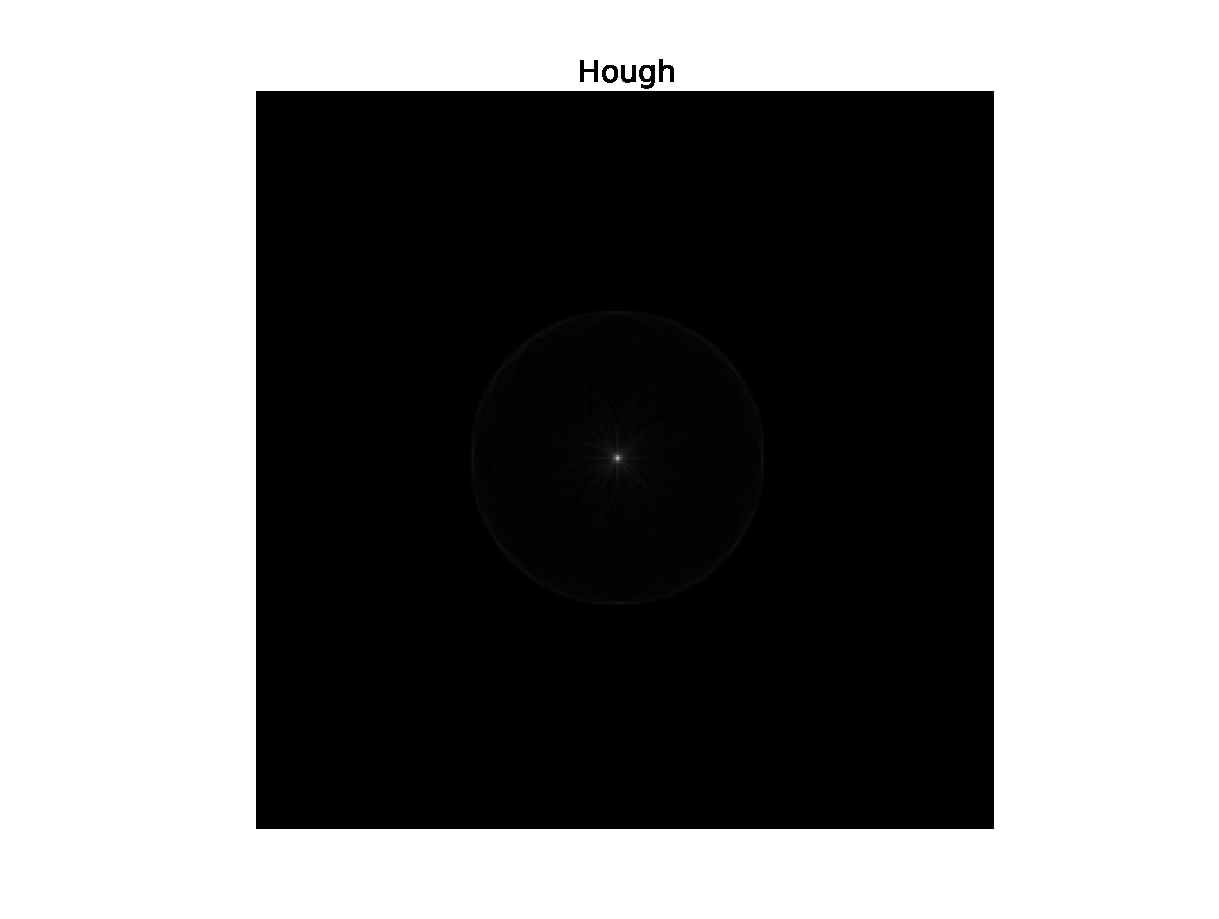
\includegraphics[width=.31\textwidth]{./figure/simple_circle_hough_img}
\label{fig:hough:simple_circle:32:weighted_vote:hough} }
\subfigure[Hough space after weighted revoting]{
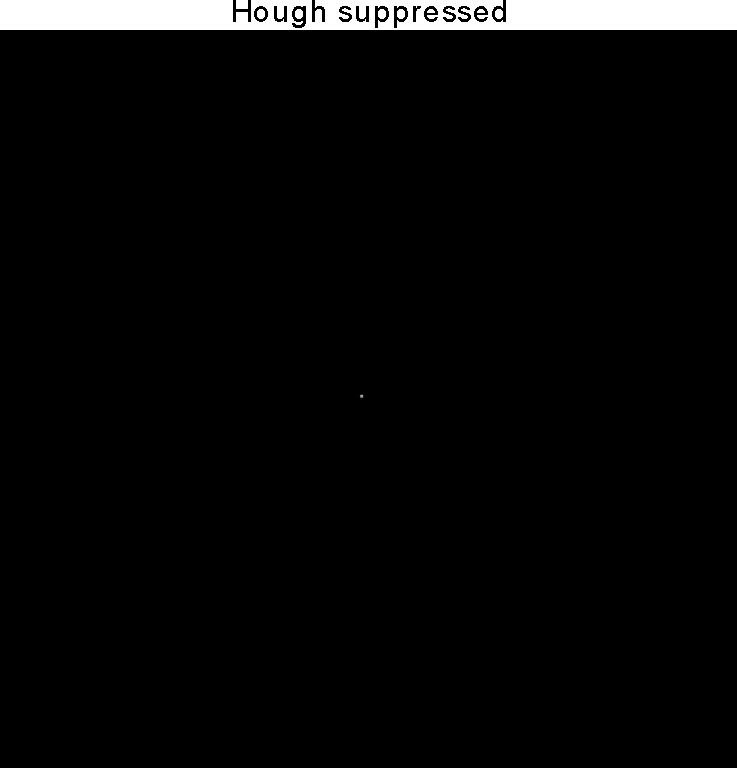
\includegraphics[width=.31\textwidth]{./figure/simple_circle_hough_img_sup} 
\label{fig:hough:simple_circle:32:weighted_vote:hough_sup} } 
\subfigure[Circles found]{
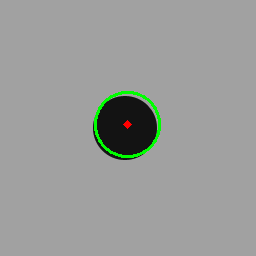
\includegraphics[width=.31\textwidth]{./figure/simple_circle_pgm_circles_32_revote}
\label{fig:hough:simple_circle:32:weighted_vote:circles} }
\caption{Detecting circles (radius=32) on \emph{circles.ppm} using weighted revote.}
\label{fig:hough:simple_circle:32:weighted_vote}
\end{figure}

Figure \ref{fig:hough:simple_circle:32:weighted_vote} gives the application on a simple case. 
As shown in Figure \ref{fig:hough:simple_circle:32:weighted_vote:hough_sup}, the most likely parameter has been strengthened and the other parameters have been weakened by this revote process.
A simple threshold can be applied to find the parameter in this case, which is shown in Figure \ref{fig:hough:simple_circle:32:weighted_vote:circles}.

\begin{figure}[h]
\centering
\subfigure[Hough space]{
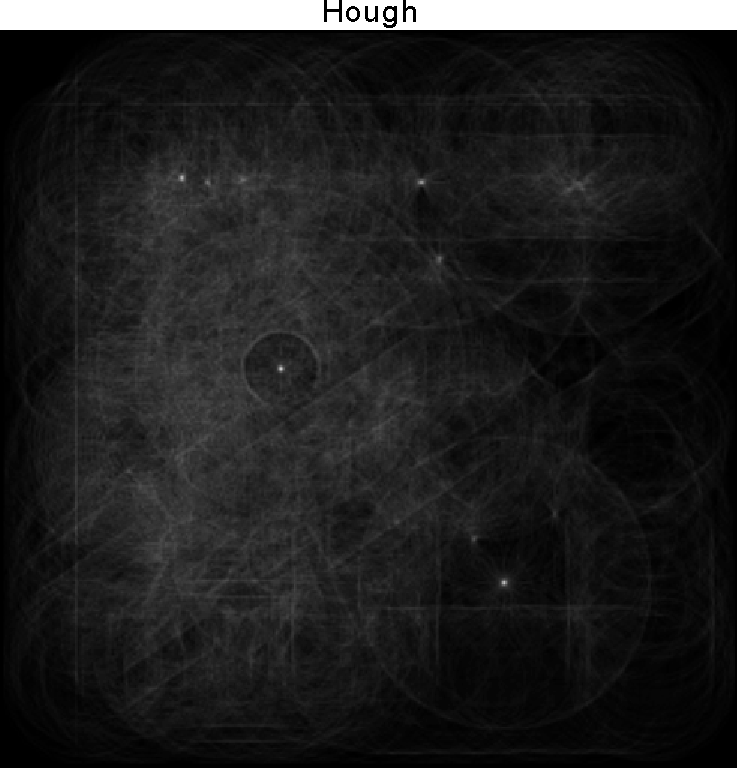
\includegraphics[width=.31\textwidth]{./figure/circles_hough_img}
\label{fig:hough:circle:32:weighted_vote:hough} }
\subfigure[Hough space after weighted revoting]{
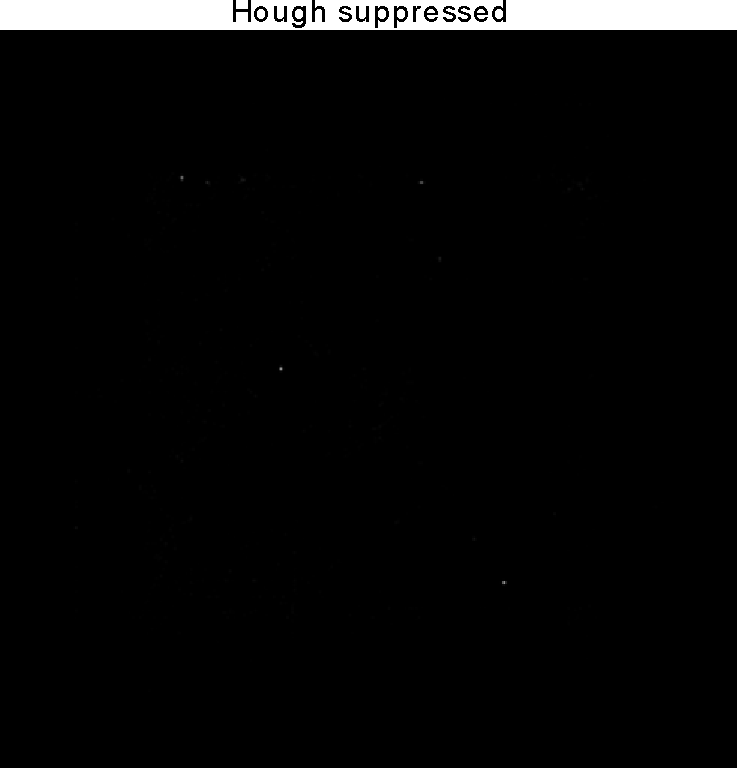
\includegraphics[width=.31\textwidth]{./figure/circles_hough_img_sup} 
\label{fig:hough:circle:32:weighted_vote:hough_sup} } 
\subfigure[Circles found]{
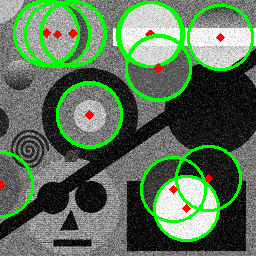
\includegraphics[width=.31\textwidth]{./figure/circles_ppm_circles_32_revote}
\label{fig:hough:circle:32:weighted_vote:circles} }
\caption{Detecting circles (radius=32) on \emph{circles.ppm} using weighted revote.}
\label{fig:hough:circle:32:weighted_vote}
\end{figure}

For normalized data array (between 0.0 and 1.0) after a bunch of weighted revote process, applying a small threshold of only $ 0.06 $ can return a set of centers found for circles with radius = 32 , which are (46, 32), (46, 33), (72, 33), (73, 33), (57, 34), (149, 34), (150, 34), (151, 34), (220, 37), (158, 67), (158, 68), (89, 114), (89, 115), (208, 178), (0, 184), (173, 189), (186, 208).
The visualized results are given in Figure \ref{fig:hough:circle:32:weighted_vote}.
This result significantly beats the results given in Figure \ref{fig:hough:circle:32:circles} and Figure \ref{fig:hough:circle:32:cv:circles}.

The revote process takes very little time. 
However, constructing the ``Bayesian'' network for the edge points (evidence) and the accumulators take pretty much time.
Due to the limitation of time, finding different size of radii at the same time is not tested.

\subsection{Discussion}

\begin{itemize}
\item \emph{ Choose different set of edge points to find the features with different size. } \\
The threshold chosen for edge detection has impact on the feature detection. 
Different sets of edge points might provide significantly different clues which support different features.
In detecting radius = 64, I choose to allow more details on the edges so that the circle of the ``face'' can be detected.
\item \emph{ Weighted revote works good but take longer time. } 
The revote process successfully strengthens the ``strong'' accumulators and suppresses the ``weak'' accumulators.
Constructing the data structure of the relationships between accumulators and edge points requires more processing time.
\end{itemize}


\end{document}